% Copyright (c) 2014,2016 Casper Ti. Vector
% Public domain.
\chapter{KV Framework底层管理接口设计}
% \pkuthssffaq % 中文测试文字。
% vim:ts=4:sw=4
\section{概览}\label{sec:Overview}
	这章将描述底层管理接口设计,包括KVF接口,Pool接口,对象接口。KVF的相关函数名称都以“KVF\_”开始。
\section{基本数据结构}\label{sec:KVF-Basic-Data-Structure}
	
	\subsection{基本数据结构}
		\begin{center}
			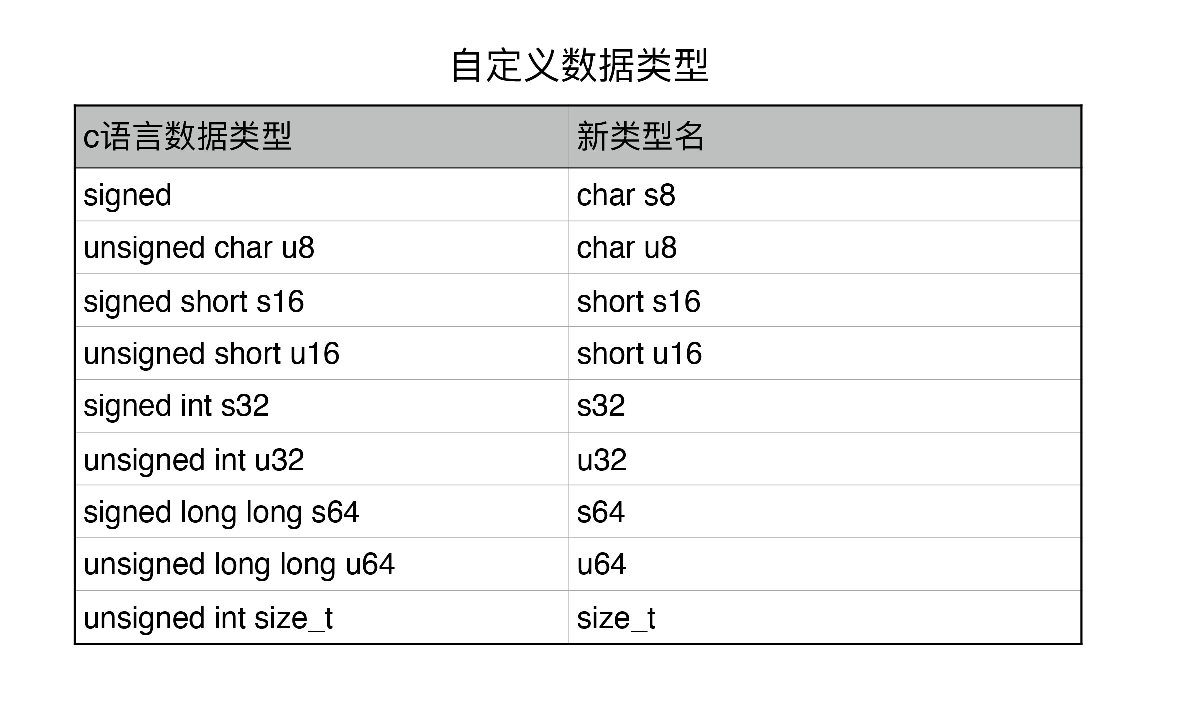
\includegraphics[width=13.9cm]{img/figure4.pdf}
		\end{center}
	\subsection{字符串结构定义}
		\begin{center}
			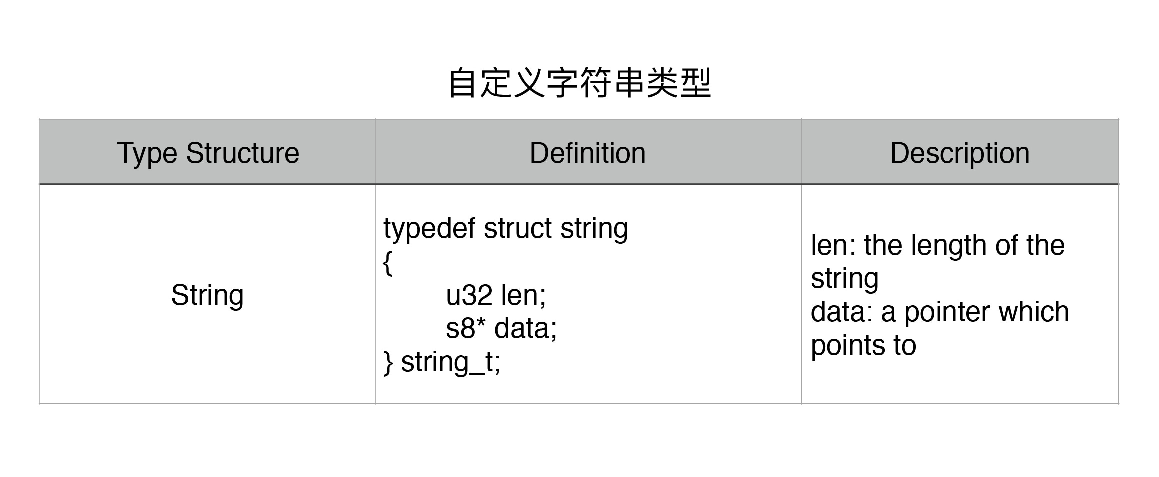
\includegraphics[width=13.9cm]{img/figure5.pdf}
		\end{center}

\section{KVF注册和注销接口}
	\begin{Verbatim}[frame = none]
    s32 kvf_register(kvf_type_t * kvf)
	\end{Verbatim}
	\begin{Verbatim}[frame = none]
    s32 kvf_unregister(kvf_type_t * kvf)
	\end{Verbatim}
		

	这两个接口使得厂商可以注册和注销自己的键值存储到KVF中,相关信息应该存储在kvf\_type\_t数据结构中,是开发者必须实现的函数。

	kvf\_type\_t结构定义如下

	\begin{center}
		\includegraphics[width=13.9cm]{img/figure6.pdf}
	\end{center}
\section{KV-LIB 接口}
	KV-LIB是厂商指定的键值库,通过这个键值库,厂商可以管理键值存储,包括初始化、关闭、设置属性等待。
	\subsection{kvf\_init()}
		该函数用于初始化KVF
		\begin{Verbatim}[frame = none]
    s32 kvf_init(const char * config_file)
		\end{Verbatim}

		参数说明:
			
			configure\_file:是指定的配置文件的目录
	\subsection{kvf\_shutdown ()}
		该函数用于关闭KVF
			
		\begin{Verbatim}[frame = none]
    s32 kvf_shutdown()
		\end{Verbatim}

		参数说明:
		\begin{itemize}
			\item \verb||
				此函数没有参数
		\end{itemize}
		% \begin{itemize}
		% 	\item \verb|copyright.tex|:版权声明部分。
		% 	\item \verb|originauth.tex|:
		% 		原创性声明和使用授权说明部分\supercite{pku-originauth}。
		% \end{itemize}

	\subsection{kvf\_set\_prop()}
		该函数用于设置KVF的相关属性值
		\begin{Verbatim}[frame = none]
    s32 kvf_set_prop(const char* name, const char* value)		
		\end{Verbatim}
		

		参数说明:
		\begin{itemize}
		\item \verb|name|:
			是指相关属性的名称
		\item \verb|value|:
			是相关属性的值
		\end{itemize}

	\subsection{kvf\_get\_prop()}
		该函数用于获得KVF的相关属性值
		\begin{Verbatim}[frame = none]
    s32 kvf_get_prop(const char* name, const char* value)		
		\end{Verbatim}
		

		参数说明:
		\begin{itemize}
		\item \verb|name|:
			是指相关属性的名称
		\item \verb|value|:
			是相关属性的值
		\end{itemize}
	
	\subsection{kvf\_alloc\_buf()}
		该函数用于在内存中分配一段数据缓冲区
		\begin{Verbatim}[frame = none]
    void* kvf_alloc_buf (size_t size, s32 flag)		
		\end{Verbatim}
		
		参数说明:
		\begin{itemize}
		\item \verb|size|:
			是需要的缓冲区空间大小
		\item \verb|flag|:
			是相关属性的值
		\end{itemize}
		
	\subsection{kvf\_free\_buf()}
		该函数用于在内存中释放数据缓冲区
		\begin{Verbatim}[frame = none]
    void* kvf_free_buf (void** buf)		
		\end{Verbatim}
		
		参数说明:
		\begin{itemize}
		\item \verb|buf|:
			需要释放内存空间的指针
		
		\end{itemize}
		
	\subsection{kvf\_get\_errstr()}
		该函数用于根据错误代码得到描述错误问题的字符串
		
		\begin{Verbatim}[frame = none]
    const char* kvf_get_errstr (s32 err_code)		
		\end{Verbatim}
		
		参数说明:
		\begin{itemize}
		\item \verb|err_code|:
			错误代码
		
		\end{itemize}

	\subsection{kvf\_get\_stats()}
		该函数u 用语获得KVF的统计数据

		\begin{Verbatim}[frame = none]
    s32 kvf_get_stats (kvf_stats_t* kvfstats)		
		\end{Verbatim}
		
		参数说明:
		\begin{itemize}
		\item \verb|kvfstats|:
			传入该kvf\_stats\_t结构的指针,函数体将数据写入该指针所指向的内存地址
		
		\end{itemize}

	% \subsection{kvf\_trans\_start()}
	% 	s32 kvf\_trans\_start(kv\_trans\_id\_t ** t\_id)
	% 	参数说明:
	% 		name是指相关参数的名词
	% 		value是相关参数的值
	% \subsection{kvf\_trans\_commit()}
	% 	s32 kvf\_trans\_commit(kvf\_trans\_id\_t* t\_id)
	% 	参数说明:
	% 		name是指相关参数的名词
	% 		value是相关参数的值
	% \subsection{kvf\_trans\_abort()}
	% 	s32 kvf\_trans\_abort(kvf\_trans\_id\_t* t\_id)
	% 	参数说明:
	% 		name是指相关参数的名词
	% 		value是相关参数的值

\section{POOL接口}
	在KVF-LIB注册并初始化之后,pool才能被管理。
	pool\_t的结构体定义如下:
	\begin{center}
		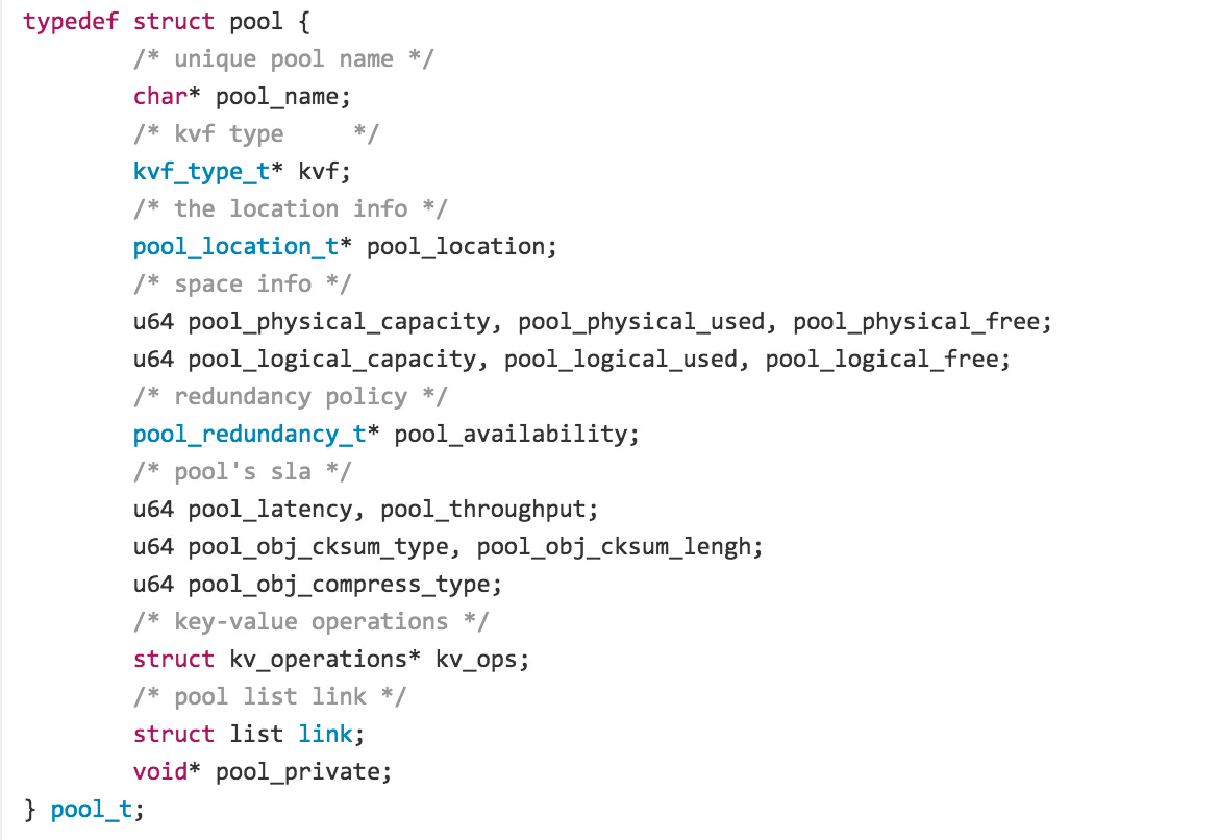
\includegraphics[width=13.9cm]{img/figure7.pdf}
	\end{center}
	\subsection{pool\_create()}
		用于创建新的pool
		\begin{Verbatim}[frame = none]
    s32 pool_create (const char* name, const char* config_path, 
		    pool_t * pool)	
		\end{Verbatim}

		参数说明:
		\begin{itemize}
		\item \verb|name|:
			指定pool的名称,每个KVF里的pool的name须唯一
		\item \verb|config_path|:
			指定相关配置文件的路径
		\item \verb|pool|:
			传入pool\_t结构指针,函数体将数据写入该指针所指向的内存地址		
		\end{itemize}
		

	\subsection{pool\_destroy()}
		销毁一个pool
		\begin{Verbatim}[frame = none]
    s32 pool_destroy (pool_t * pool)
		\end{Verbatim}

		参数说明:
		\begin{itemize}
		\item \verb|pool|:
			传入pool\_t结构指针,函数体将数据写入该指针所指向的内存地址
		\end{itemize}


	\subsection{pool\_open()}
		打开一个pool
		\begin{Verbatim}[frame = none]
    s32 pool_open (pool_t * pool)
		\end{Verbatim}		

		参数说明:
		\begin{itemize}
		\item \verb|pool|:
			传入pool\_t结构指针,函数体将数据写入该指针所指向的内存地址
		\end{itemize}


	\subsection{pool\_close()}
		关闭一个pool
		\begin{Verbatim}[frame = none]
    s32 pool_close (pool_t * pool)
		\end{Verbatim}		

		参数说明:
		\begin{itemize}
		\item \verb|pool|:
			传入pool\_t结构指针,函数体将数据写入该指针所指向的内存地址
		\end{itemize}


	\subsection{pool\_set\_prop()}
		设置pool的相关属性
		\begin{Verbatim}[frame = none]
    s32 pool_set_prop (const pool_t * pool,const char* name, 
			    const char* value )
		\end{Verbatim}

		参数说明:
		\begin{itemize}
		\item \verb|pool|:
			传入pool\_t结构指针,函数体将数据写入该指针所指向的内存地址,该参数是常量
		\item \verb|name|:
			需要设置的属性名称
		\item \verb|value|:
			需要设置的属性值
		\end{itemize}
	\subsection{pool\_get\_prop()}
		获取指定pool属性的值
		\begin{Verbatim}[frame = none]
    s32 pool_get_prop (const pool_t * pool,const char* name, 
			    const char* value )
		\end{Verbatim}

		参数说明:
		\begin{itemize}
		\item \verb|pool|:
			传入pool\_t结构指针,函数体将数据写入该指针所指向的内存地址,该属性是常量
		\item \verb|name|:
			需要设置的属性名称
		\item \verb|value|:
			需要设置的属性值
		\end{itemize}

	\subsection{pool\_get\_stats()}
		获取pool的统计数据
		\begin{Verbatim}[frame = none]
    s32 pool_set_stats (pool_stats_t * stats)
		\end{Verbatim}		

		参数说明:
		\begin{itemize}
		\item \verb|stats|:
			传入pool\_stats\_t结构指针,函数体将数据写入该指针所指向的内存地址
		\end{itemize}
	
	\section{对象键值接口}
		在pool成功创建之后,我们可以操作属于于该pool的对象

		\subsection{put}
			将数据写入磁盘
		\begin{Verbatim}[frame = none]
    s32 put(pool_t* pool,const string_t* key, const string_t* value,
	    const kv_props_t* props, const put_options_t* putopts)
		\end{Verbatim}

		参数说明:
		\begin{itemize}
		\item \verb|pool|:
			传入pool\_t结构指针,函数体将数据写入该指针所指向的内存地址,该参数是常量
		\item \verb|key|:
			需要写入的键
		\item \verb|value|:
			需要写入的属性值
		\item \verb|props|:
			设置键值的属性
		\item \verb|putopts|:
			设置写入模式
		\end{itemize}

		相关结构定义:
		\begin{center}
			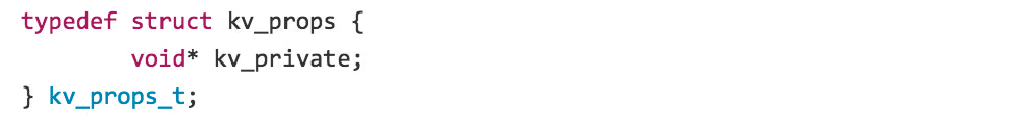
\includegraphics[width=13.9cm]{img/figure8.pdf}
		\end{center}
		\begin{center}
			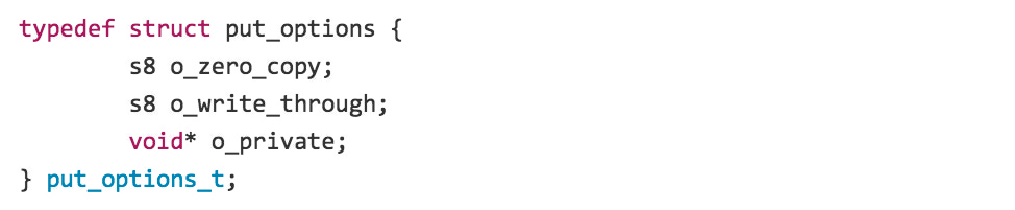
\includegraphics[width=13.9cm]{img/figure9.pdf}
		\end{center}


		\subsection{get}
			从磁盘中根据键获取值
		\begin{Verbatim}[frame = none]
    s32 get(pool_t* pool, const string_t* key, string_t* value, 
	    const kv_props_t* props, const get_options_t* getopts)
		\end{Verbatim}

		参数说明:
		\begin{itemize}
		\item \verb|pool|:
			传入pool\_t结构指针,函数体将数据写入该指针所指向的内存地址,该参数是常量
		\item \verb|key|:
			需要写入的键
		\item \verb|value|:
			该参数是string\_t结构指针,会将读取的值放入这个指针所指向的地址
		\item \verb|props|:
			设置键值的属性
		\item \verb|putopts|:
			设置写入模式
		\end{itemize}


		\subsection{del}
			从磁盘中根据键删除值
		\begin{Verbatim}[frame = none]
    s32 del(pool_t* pool, const string_t* key, const kv_props_t* props, 
        const del_options_t* delopts)
		\end{Verbatim}

		参数说明:
		\begin{itemize}
		\item \verb|pool|:
			传入pool\_t结构指针,函数体将数据写入该指针所指向的内存地址,该参数是常量
		\item \verb|key|:
			需要设置的属性名称
		\item \verb|value|:
			需要设置的属性值
		\item \verb|props|:
			设置键值的属性
		\item \verb|delopts|:
			设置写入模式
		\end{itemize}

		\subsection{iter\_open}
			根据正则表达式查询
		\begin{Verbatim}[frame = none]
    s32 iter_open(const pool_t* pool, const string_t* key_regex, 
        s32 limit, s32 timeout, kv_iter_t* it)
		\end{Verbatim}

		参数说明:
		\begin{itemize}
		\item \verb|pool|:
			传入pool\_t结构指针,函数体将数据写入该指针所指向的内存地址,该参数是常量
		\item \verb|key_regex|:
			需要查询的键的正则表达式
		\item \verb|limit|:
			查询次数的上限
		\item \verb|timeout|:
			timeout
		\item \verb|it|:
			
		\end{itemize}

		\subsection{iter\_next}
			根据正则表达式查询
		\begin{Verbatim}[frame = none]
    s32 iter_next(pool_t* pool, kv_iter_t* it, kv_array_t* kvarray)
		\end{Verbatim}

		参数说明:
		\begin{itemize}
		\item \verb|pool|:
			传入pool\_t结构指针,函数体将数据写入该指针所指向的内存地址,该参数是常量
		\item \verb|it|:
			需要查询的键的正则表达式
		\item \verb|kvarray|:
			查询次数的上限
		
		\end{itemize}

		\subsection{iter\_close}
			根据正则表达式查询
		\begin{Verbatim}[frame = none]
    s32 iter_close(pool_t* pool, kv_iter_t* it)
		\end{Verbatim}

		参数说明:
		\begin{itemize}
		\item \verb|pool|:
			传入pool\_t结构指针,函数体将数据写入该指针所指向的内存地址,该参数是常量
		\item \verb|it|:
			需要查询的键的正则表达式
		
		\end{itemize}

	\section{上层接口}
		当上层应用开发时调用如下的接口即可避免重发的适配工作,KVF将会封装常用的数据库,这样上层应用就不再考虑不同数据库之间接口的差异,大大缩短开发时间。

		根据不同的抽象层次,我们将接口分为三种:KV-LIB、Pool、对象。由于大部分功能和底层接口类似,在这里我将不再详细介绍每一个函数参数的含义。
		\subsection{KVF接口}

			\begin{Verbatim}[frame = none]
    s32 kvf_init(const char * config_file) 

    kvf_type_t* get_kvf(const char* name)

    s32 init_kvf(const char * config_file)

    s32 shutdown_kvf()

    s32 set_kvf_ prop(const char* name, const char* value)

    s32 get_kvf_ prop(const char* name, char** value)

    void* alloc_kvf_ buf (size_t size, s32 flag)

    void free_kvf_ buf (void** buf)

    s32 get_kvf_ stats (kvf_stats_t* kvfstats)

    s32 start_kvf_trans (kv_trans_id_t ** t_id)

    s32 commit_kvf_trans (kvf_trans_id_t* t_id)
    
    s32 abort_kvf_trans (kvf_trans_id_t* t_id)
			\end{Verbatim}

		\subsection{Pool接口}
			\begin{Verbatim}[frame = none]
    s32 create_pool (const char* name, const char* config_path, 
    pool_t * pool)

    s32 destroy_pool (pool_t * pool)

    s32 open_pool (pool_t * pool)

    s32 close_pool (pool_t* pool)

    s32 set_pool_prop(const pool_t* pool, const char* name, 
    const char* value )

    s32 get_pool_prop(const pool_t* pool, const char* name, 
    char** value)
    s32 get_pool_stats (pool_stats_t * stats)

			\end{Verbatim}

		\subsection{Pool接口}
			\begin{Verbatim}[frame = none]
    s32 put(pool_t* pool,const string_t* key, const string_t* value,
    const kv_props_t* props, const put_options_t* putopts);

    s32 get(pool_t* pool, const string_t* key, string_t* value, 
    const kv_props_t* props, const get_options_t* getopts)

    s32 del(pool_t* pool, const string_t* key, const kv_props_t* props, 
    const del_options_t* delopts)

    s32 mput(pool_t* pool, kv_array_t* kvarray, const kv_props_t* props, 
    const put_options_t* putopts)

    s32 mget(pool_t* pool, kv_array_t* kvarray, const kv_props_t* props, 
    const get_options_t* getopts)

    s32 mdel(pool_t* pool, array_t* kvarray, const kv_props_t* props, 
    const del_options_t* delopts)

    s32 open_iter (const pool_t* pool, const string_t* key_regex, 
    s32 limit, s32 timeout, kv_iter_t* it)

    s32 next_iter (pool_t* pool, kv_iter_t* it, 
    kv_array_t* kvarray)

    s32 close_iter (pool_t* pool, kv_iter_t* it)

    s32 xcopy_obj(const pool_t* src, const pool_t* dest,
    const string_t* regex)

			\end{Verbatim}